
\section{Création du serveur CLI}
Pour le serveur Jenkins, on a décidé d'utiliser une Machine Virtuelle tournant sur \textit{VirtualBox} et utilisant une image \textit{Ubuntu Server}.
Nous avons des machines personnelles tournant sous Linux, donc nous n'avions pas accès à WSL, ceci étant donné, cette solution offrait un bon compromis entre taille de la VM et rapidité de configuration.\\

Comme nous utilisions une machine virtuelle locale et que nous allons avoir besoin d'accéder à des services internet sur celle-ci (Serveur Web, SSH), il a fallu jouer avec les paramètres réseau de VirtualBox.
Heureusement, VirtualBox propose de gérer le NAT du routeur virtuel sur lequel est interfacé notre VM\@.
Ainsi, on a pu exposer le port 9090 (HTTP utilisé par Jenkins) de la VM sur le port 9090 du réseau local, et le port 22 (SSH) sur le port 2222\@ (fig.~\ref{fig:NAT}).
Ceci étant fait après avoir ouvert le pare-feu de la VM (avec \textit{sudo ufw enable ssh}), nous allons pouvoir nous connecter via SSH à la VM et profiter du confort de notre interface locale.\\

\begin{figure}[h]
    \centering
    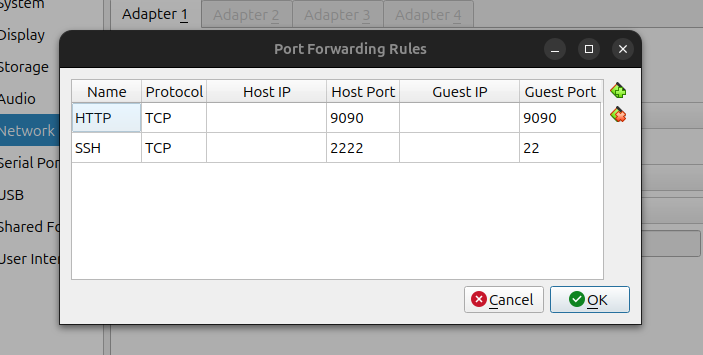
\includegraphics[width=.5\textwidth]{serveur-cli/NAT}
    \caption{Configuration du port forwarding de notre VM}
    \label{fig:NAT}
\end{figure}


Ensuite, en suivant les instructions données pour l'installation de Jenkins (installation et démarrage du service, déploiement des clés SSH). Nous pouvons accéder au tableau de bord du service.
Etant donnée notre configuration utilisant un NAT, on accède pas à ce service via l'adresse IP de l'interface \textit{eth0} de la VM mais via l'adresse \textit{localhost (127.0.0.1)}.
Une fois connectés, on a du relancer plusieurs fois l'installation de tous les plugins, mais tout a fini par se finir correctement.\\

Ensuite, on a pu mettre en place la pipeline en permettant à Jenkins d'utiliser le JenkinsFile de notre repo Github sans problème\@.
On a pu enfin la lancer pour la première fois et vérifier que tout fonctionnait proprement (fig.~\ref{fig:PipelineFailed})

\begin{figure}[h]
    \centering
    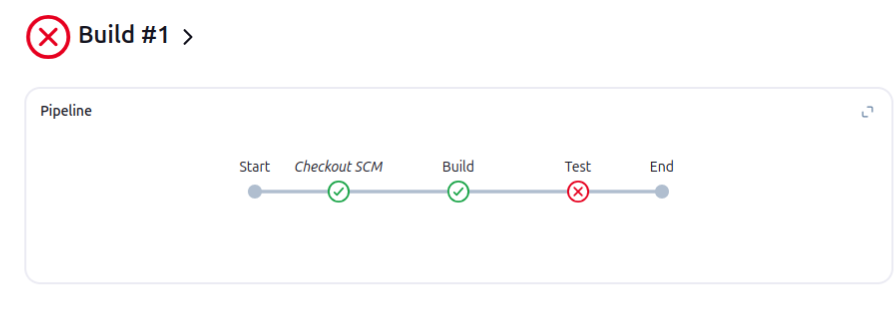
\includegraphics[width=.7\textwidth]{serveur-cli/PipelineFailed}
    \caption{Task Failed successfully!!}
    \label{fig:PipelineFailed}
\end{figure}


